\documentclass[tikz, border=2pt]{standalone}
\usepackage{tikz}
\usetikzlibrary{arrows.meta, positioning, calc}

% --- 沿用模板配色 ---
\definecolor{WLTeal}{HTML}{00897B}   
\definecolor{WLOrange}{HTML}{FF7043} 
\definecolor{WLGray}{HTML}{546E7A}   

\begin{document}
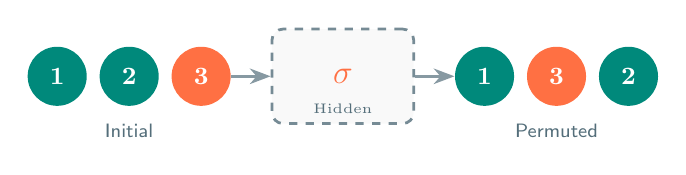
\begin{tikzpicture}[
    % 全局缩放与间距设置
    node distance=0.15cm, % 极小间距
    font=\sffamily,
    % 样式定义
    ball/.style={
        circle, 
        minimum size=0.75cm, % 缩小球体尺寸
        inner sep=0pt, 
        text=white, 
        font=\bfseries\small, % 字体改小
        draw=none
    },
    blueball/.style={ball, fill=WLTeal},
    redball/.style={ball, fill=WLOrange},
    labeltext/.style={font=\scriptsize\sffamily, text=WLGray, align=center}
]

    % ====== 1. 中间:置换算符 (核心锚点) ======
    \node[
        draw=WLGray!80, 
        dashed, 
        line width=1pt,
        rounded corners=4pt,
        minimum width=1.8cm, 
        minimum height=1.2cm,
        fill=gray!5
    ] (sigma) at (0,0) {};
    
    \node[text=WLOrange, font=\large\bfseries] at (sigma.center) {$\sigma$};
    \node[text=WLGray, font=\tiny, below=0.2em of sigma.center] at (0,-0.15) {Hidden};

    % ====== 2. 左侧:初始状态 (两蓝一红) ======
    % 这里的坐标是相对于中间方块计算的,非常紧凑
    \node[redball]  (L3) [left=0.5cm of sigma] {3};
    \node[blueball] (L2) [left=of L3] {2};
    \node[blueball] (L1) [left=of L2] {1};
    
    % 连接箭头
    \draw[->, >={Stealth[scale=1]}, line width=1pt, WLGray!70] (L3.east) -- (sigma.west);
    
    % 底部标签
    \node[labeltext, below=0.1cm of L2] {Initial};

    % ====== 3. 右侧:置换后状态 (红球位置改变) ======
    % 例子:位置2和位置3互换 (Odd Permutation)
    % 现在的顺序是: 1(蓝), 3(红), 2(蓝)
    \node[blueball] (R1) [right=0.5cm of sigma] {1};
    \node[redball]  (R2) [right=of R1] {3}; % 红球换到了中间
    \node[blueball] (R3) [right=of R2] {2}; % 蓝球换到了后面
    
    % 连接箭头
    \draw[->, >={Stealth[scale=1]}, line width=1pt, WLGray!70] (sigma.east) -- (R1.west);

    % 底部标签
    \node[labeltext, below=0.1cm of R2] {Permuted};

\end{tikzpicture}
\end{document}